\section{Auswertung}
\label{sec:Auswertung}

Die Graphen werden sowohl mit Matplotlib \cite{matplotlib} als auch NumPy \cite{numpy} erstellt. Die Fehlerrechnung wird mithilfe von Uncertainties \cite{uncertainties} durchgeführt.

\subsection{Bestimmung der mittleren Weglänge}

Mit den Werten der Temperaturen $T$ aus Tabelle \ref{tab:w} ergeben sich die mittleren Weglängen $\bar{w}$ nach Formel \eqref{eq:w}. Das Verhältnis von $\bar{w}$ zum Abstand $a=\SI{1}{\centi\metre}$ der Kathode zum Gitter ist ebenfalls in der Tabelle eingetragen. 

\begin{table}
\centering
\caption{[ToDo].}
\label{tab:tabw}
	\sisetup{table-format=1.2}
	\begin{tabular}{S[table-format=3.2]cc}
		\toprule
		{$T/\si{\kelvin}$} & {$\bar{w}/\si{\metre}$} & {$\frac{a}{\bar{w}}$} \\
		\midrule
		 296,65 & 6,14$\cdot10^{-3}$ & 1,63$\cdot10^{0}$ \\
		 417,15 & 7,60$\cdot10^{-6}$ & 1,32$\cdot10^{3}$ \\
		 447,35 & 2,50$\cdot10^{-6}$ & 4,01$\cdot10^{3}$ \\
		 381,15 & 3,60$\cdot10^{-5}$ & 2,77$\cdot10^{2}$ \\
		\bottomrule
	\end{tabular}

\label{tab:w}
\end{table}

\subsection{Bestimmung der Umrechnungsfaktoren}

Für die X-Achse der Graphen aus den Abbildungen \ref{fig:} bis \ref{fig:} werden die Umrechnungsfaktoren bestimmt.
Mit den Werten aus Tabelle \ref{tab:Abstände} und der Formel für den Mittelwert
\[
\mu_d = 
\]
und der Standardabweichung
\[
\sigma_d = 
\]
ergeben sich die mittleren Abstände $\bar{d}$ pro Volt zu:
\begin{align*}
\bar{d}_.{a1} &= \SI{24.8(4)}{\milli\metre\per\volt}\text{,}\\
\bar{d}_.{a2} &= \SI{25.1(4)}{\milli\metre\per\volt}\text{,}\\
\bar{d}_.{b}  &= \SI{4.6(2)}{\milli\metre\per\volt}\text{,}\\
\bar{d}_.{c}  &= \SI{7.7(2)}{\milli\metre\per\volt}\text{.}
\end{align*}
Daraus folgen die Umrechnungsfaktoren $f=\frac{1}{\bar{d}}$ zu:
\begin{align}
f_.{a1} &= \SI{40.3(6)}{\volt\per\metre}\text{,}\\
f_.{a2} &= \SI{39.8(6)}{\volt\per\metre}\text{,}\\
f_.{b}  &= \SI{217(9)}{\volt\per\metre}\text{,}\\
f_.{c}  &= \SI{130(3)}{\volt\per\metre}\text{.}
\end{align}
Der Fehler $\sigma_{f}$ zu $f$ berechnet sich dabei mit der Gaußschen Fehlerfortpflanzung nach:
\[
\sigma_{f} = 
\]

\begin{table}
\centering
\caption{[ToDo].}
\label{tab:tabAbstaende}
	\sisetup{table-format=1.2}
	\begin{tabular}{S[table-format=2.0]S[table-format=2.0]S[table-format=1.1]S[table-format=1.1]}
		\toprule
		{$d_\text{a1}/(\si{\milli\metre\per\volt})$} & {$d_\text{a2}/(\si{\milli\metre\per\volt})$} & {$d_\text{b}/(\si{\milli\metre\per\volt})$} & {$d_\text{c}/(\si{\milli\metre\per\volt})$} \\
		\midrule
		24 & 25 & 4.8 & 8.6 \\
		25 & 24 & 3.6 & 8.0 \\
		23 & 26 & 4.4 & 7.0 \\
		26 & 24 & 4.8 & 7.0 \\
		24 & 23 & 5.6 & 7.0 \\
		23 & 26 & 4.6 & 8.0 \\
		25 & 25 & 4.6 & 8.2 \\
		26 & 26 & 3.6 & 7.8 \\
		26 & 26 & 5.6 & 7.8 \\
		26 & 26 & 4.8 & 7.4 \\
		 {-}  &  {-}  & 4.4 &  {-}  \\
		\bottomrule
	\end{tabular}

\label{tab:Abstände}
\end{table}

\subsection{Bestimmung der Energieverteilung der Elektronen}

Es ergibt sich ein Wert für das Kontaktpotential $k_.A$ von:
\[
k_.A = \SI{2,1(1)}{\volt}
\]

\begin{figure}
\centering
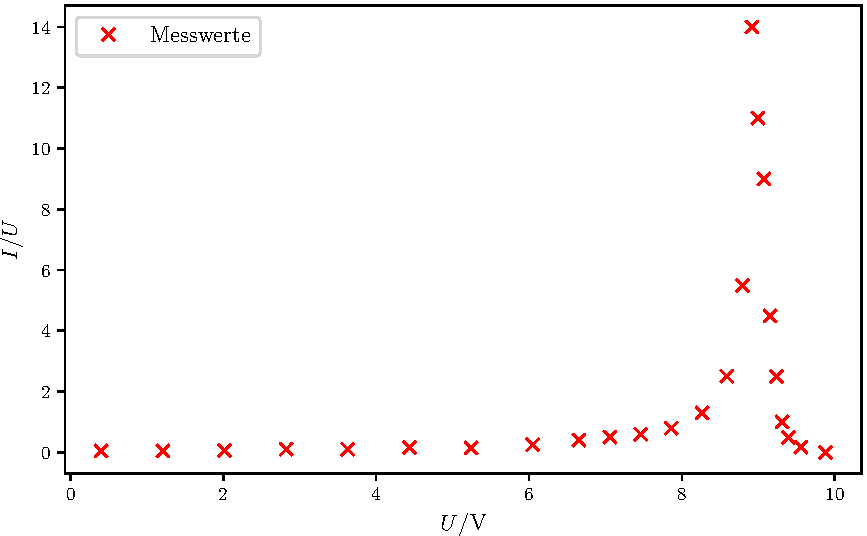
\includegraphics[width=\linewidth-70pt,height=\textheight-70pt,keepaspectratio]{content/images/fig1.pdf}
\caption{Die nicht normierte Energieverteilung der Elektronen bei einer Temperatur von $T=\SI{296,65}{\kelvin}$ und einer Beschleunigungsspannung von $U_.B=\SI{11}{\volt}$.}
\label{fig:1}
\end{figure}

\begin{figure}
\centering
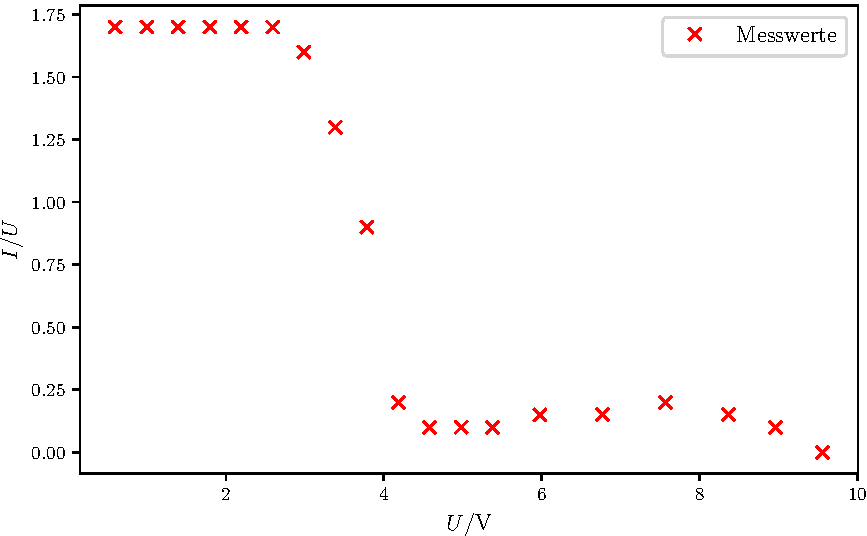
\includegraphics[width=\linewidth-70pt,height=\textheight-70pt,keepaspectratio]{content/images/fig2.pdf}
\caption{Die nicht normierte Energieverteilung der Elektronen bei einer Temperatur von $T=\SI{417,15}{\kelvin}$ und einer Beschleunigungsspannung von $U_.B=\SI{11}{\volt}$.}
\label{fig:2}
\end{figure}

\begin{table}
\centering
\caption{[ToDo].}
\label{tab:tabEnergieverteilung}
	\sisetup{table-format=1.2}
	\begin{tabular}{S[table-format=1.2]S[table-format=2.2]S[table-format=1.2]S[table-format=1.2]}
		\toprule
		{$U_.{A1}/\si{\volt}$} & {$I_1/U_.{A1}$} & {$U_.{A2}/\si{\volt}$} & {$I_2/U_.{A2}$} \\
		\midrule
		0.40 & 0.05 & 0.60 & 1.70 \\
		1.21 & 0.05 & 1.00 & 1.70 \\
		2.02 & 0.05 & 1.39 & 1.70 \\
		2.82 & 0.10 & 1.79 & 1.70 \\
		3.63 & 0.10 & 2.19 & 1.70 \\
		4.44 & 0.15 & 2.59 & 1.70 \\
		5.24 & 0.15 & 2.99 & 1.60 \\
		6.05 & 0.25 & 3.39 & 1.30 \\
		6.65 & 0.40 & 3.78 & 0.90 \\
		7.06 & 0.50 & 4.18 & 0.20 \\
		7.46 & 0.60 & 4.58 & 0.10 \\
		7.86 & 0.80 & 4.98 & 0.10 \\
		8.27 & 1.30 & 5.38 & 0.10 \\
		8.59 & 2.50 & 5.98 & 0.15 \\
		8.79 & 5.50 & 6.77 & 0.15 \\
		8.91 & 14.00 & 7.57 & 0.20 \\
		8.99 & 11.00 & 8.37 & 0.15 \\
		9.07 & 9.00 & 8.96 & 0.10 \\
		9.15 & 4.50 & 9.56 & 0.00 \\
		9.23 & 2.50 &  {-}  &  {-}  \\
		9.31 & 1.00 &  {-}  &  {-}  \\
		9.40 & 0.50 &  {-}  &  {-}  \\
		9.56 & 0.17 &  {-}  &  {-}  \\
		9.88 & 0.00 &  {-}  &  {-}  \\
		\bottomrule
	\end{tabular}

\label{tab:Energieverteilung}
\end{table}

\subsection{Bestimmung der ersten Anregungsenergie von Quecksilber}

Es ergibt sich eine Anregungsenergie $E_1$ von:
\[
E_1 = \SI{4,92(2)}{\electronvolt}
\]
Für die Wellenlänge folgt:
\[
\lambda = \SI{252(1)}{\nano\metre}
\]

\subsection{Bestimmung der Ionisierungsenergie von Quecksilber}

Es ergibt sich eine Ionisierungsenergie von:
\[
E_.{Io,1} = \SI{15.6(1)}{\electronvolt}
\]
Unter großzügiger auslegung der Asymptote ergibt sich:
\[
E_.{Io,2} = \SI{12.9(1)}{\electronvolt}
\]